\documentclass[xcolor=dvipsnames]{beamer}
\usepackage[utf8]{inputenc}
\usepackage[IL2]{fontenc}
\usepackage[czech]{babel}
\usepackage{float}
\usepackage{listings}
\usepackage{amssymb}
\usepackage{amsmath}
\usepackage{mathtools}
\usepackage{url}
\usepackage{graphicx}
\usepackage{subfigure}
%\useoutertheme[subsection=false]{smoothbars}
\usetheme{Madrid}
\usecolortheme{crane}
%\usecolortheme[named=OliveGreen]{structure} 
%\usetheme[height=7mm]{Rochester} 
%\setbeamertemplate{items}[ball] 
%\setbeamertemplate{blocks}[rounded][shadow=true] 
%\useoutertheme{umbcfootline}
\beamertemplatenavigationsymbolsempty 
\addtobeamertemplate{block begin}{%
  \setlength{\textwidth}{0.9\textwidth}%
}{}
%\useoutertheme{umbcfootline}
%\setfootline{ \hfill\insertframenumber /\inserttotalframenumber}

\title{Design and implementation of a social network for making acquaintances}
\subtitle{Obhajoba bakalářské práce}
\author{Marek Bryša}
\date{22. června 2012}
\institute
{
Masarykova Univerzita\\
Fakulta informatiky
}
\begin{document}
  \frame{\titlepage}
	\begin{frame}{Cíle práce}
		\begin{itemize}
			\item Prozkoumat existující společenslé sítě pro vytváření známostí a vyhodnotit jejich klady a zápory
			\item Shrnout relevantní aspekty ochrany osobních údajů v těchto sítích
			\item Narhnout novou společenskou síť
			\item Zvolit nejvhodnější technologie pro implementaci
			\item Implementovat prototyp
			\item Popsat implementaci s uživatelského a programátorského pohledu
		\end{itemize}
	\end{frame}
	\begin{frame}{Existující společenské sítě}
		PlentyofFish, Match.com, OkCupid, eHarmony,...\\
		\bigskip
		Společné vlastnosti:
		\begin{itemize}
			\item Nutno vyplňovat zdlouhavé dotazníky citlivými (časti i intimními) osobními údaji\\
				$\implies$ Možnost zneužití nebo úniku těchto údajů
			\item Matematický nebo nějak "zázračný" systém na automatické vyhledání vhodného partnera\\
				Podle Finkel et al. (2012) tyto systémy stejně nefungují
			\item Nutno sebrat odvahu a iniciativně kontaktovat nalezeného partnera\\
				
		\end{itemize}
	\end{frame}
	\begin{frame}{Návrh nové společenské sítě}
		\begin{enumerate}
			\item Uživatel poskutne pouze tyto údaje:\\
		    rok narození, pohlaví, přibližná poloha na úroveň okresu, jedna fotografie
	    \item Ostatní uživatele vyhledá podle kritérií:\\
	      pohlaví, věkové rozpětí, relativní poloha (stejný okres, sousední okresy, stejný kraj, sousední kraje, stejný stát)
	    \item Prohlíží si fotografie nalezených uživatelů jednu po druhé a označuje ty, kteří se mu líbí
	    \item Pouze až se dva uživatelé označí, že se sobě vzájemně líbí, oba se o tom dozví a je jim nabídnuta možnost real-time chatu, kde se mohou dále poznat
		\end{enumerate}
	\end{frame}
	\begin{frame}{Technologie}
		\begin{figure}[htb]
	  \centering
	    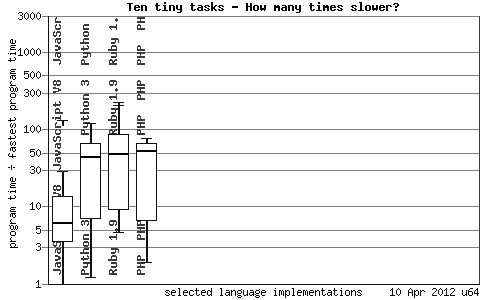
\includegraphics[width=0.8\textwidth]{../tex/bench2.png}
		  \caption{Benchmark jazyků V8 Engine, Python 3, Ruby 1.9 and PHP 5.4.0. Menší znamená ryhlejší. Zdroj: The Computer Language Benchmarks Game}
		  \label{fig:bench1}
		\end{figure}
	\end{frame}
	\begin{frame}{Technologie}
				\begin{figure}[h!]
	  \centering
	    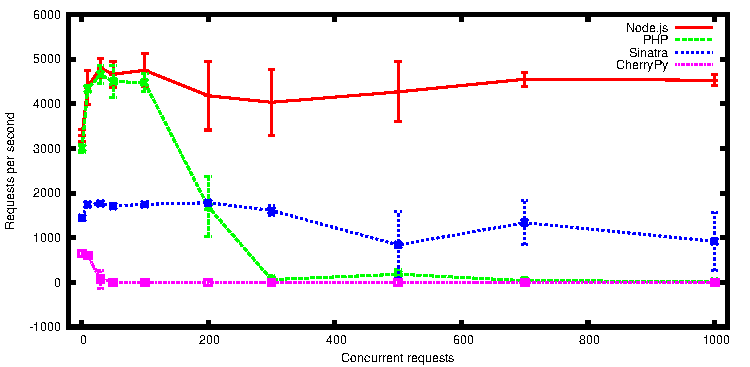
\includegraphics[width=0.9\textwidth]{../tex/plot_add.pdf}
		  \caption{Benchmark metody \texttt{add}.}
		  \label{fig:bench_add}
		\end{figure}		

	\end{frame}
	\begin{frame}{Technologie}
			\begin{figure}[h!]
	  \centering
	    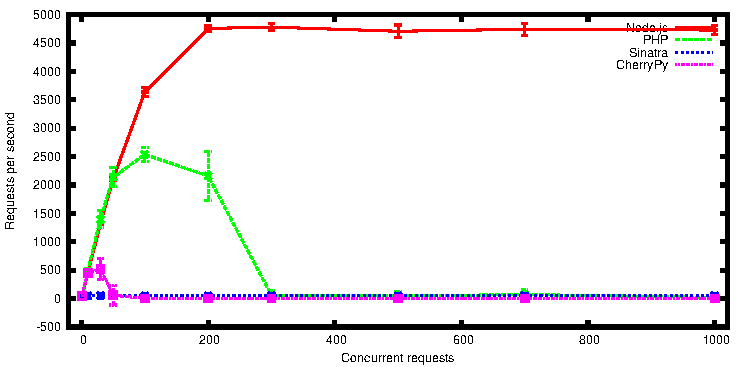
\includegraphics[width=0.9\textwidth]{../tex/plot_sleep.pdf}
		  \caption{Benchmark metody \texttt{sleep}.}
		  \label{fig:bench_sleep}
		\end{figure}
  \end{frame}
  \begin{frame}{Zvolená technologie}
  	Podle výkonu a dalších kriterií (celková vhodnost, stabilita, škálovatelnost, faktor inovace,...) byl jako základ zvolen framework Node.js a jeho HTTP nádstavbový modul Express.js. \\\bigskip
  	Jako úložiště dat byl zejména z důvodu rychlosti a inovativnosti zvolen Redis (NoSQL in-memory pokročilá key-value storage)
  \end{frame}
  \begin{frame}{Implementace}
    \begin{itemize}
    	\item Vzhledem ke zvolené technologii primární zaměření na výkon\\
    		Kompletní zpracování požadavku vyhledání v souboru 200~000 uživatelů trvá na starším serveru 2~ms\\
    		Drobné zápisy do databáze (např. označení líbí/nelíbí) do 1~ms
    	\item HTML5, CSS, kompletně AJAX -- domovská stránka uživatele se načítá pouze jednou po přihlášesní, další požadavky jsou asynchronní
    	\item Možnost ořezání nahrané fotky přímo na serveru
    	\item Real-time chat pomocí socket.io (XHR long-poll i WebSocket), e-mailové upozornění na zmeškané zprávy
    	\item Geolokační databáze Yahoo! GeoPlanet
    	\item Plně funkční implementace dostupná na \url{http://pickdo.com}
    \end{itemize}
  \end{frame}

  \begin{frame}{Screenshoty}
    \begin{figure}[h]
	  \centering
	    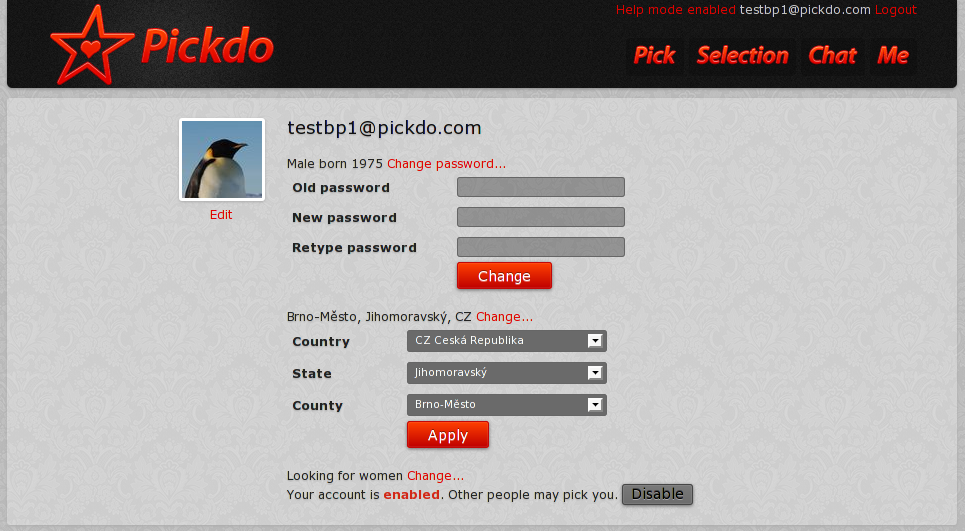
\includegraphics[width=0.9\textwidth]{../tex/screen-profile.png}
		  \caption{Stránka profilu a nastavení. (Author of the penguin photo: Hannes Grobe/AWI, CC-BY-SA 3.0)}
		  \label{fig:screen-profile}
	  \end{figure}
	\end{frame}
	
	\begin{frame}{Screenshoty}
		\begin{figure}[h]
	  \centering
	    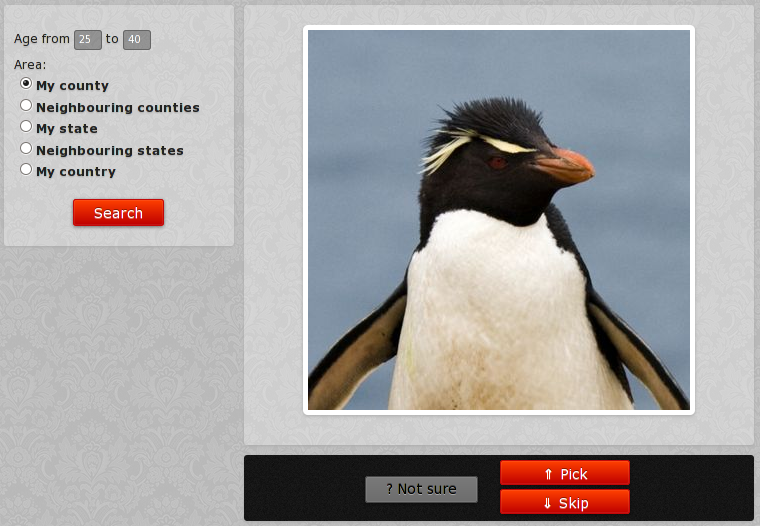
\includegraphics[width=0.8\textwidth]{../tex/screen-search.png}
		  \caption{Stránka hledání a výběru. (Author of the penguin photo: Samuel Blanc, CC-BY-SA 3.0)}
		  \label{fig:screen-search}
	  \end{figure}
	\end{frame}
	\begin{frame}{Screenshoty}
			\begin{figure}[h]
	  \centering
	    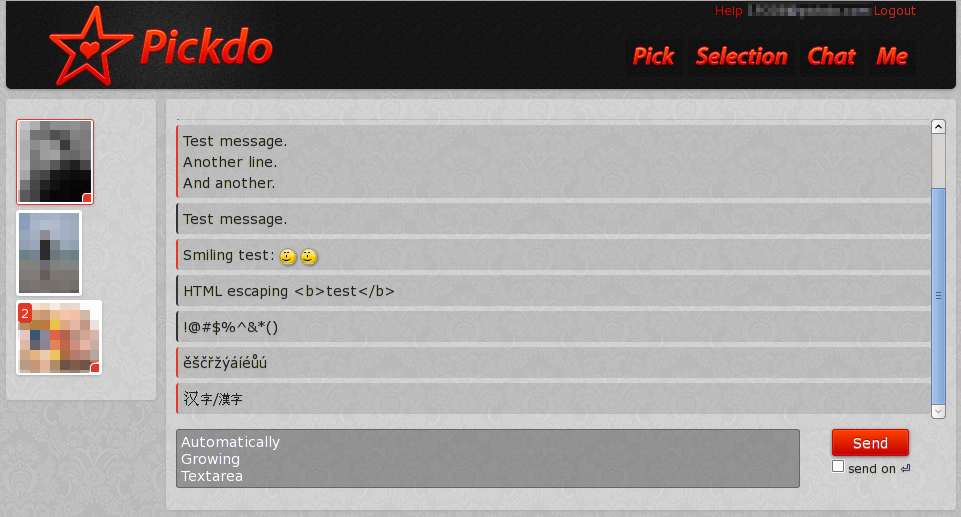
\includegraphics[width=1.0\textwidth]{../tex/screen-chat.png}
		  \caption{Stránka real-time chatu}
		  \label{fig:screen-chat}
	  \end{figure}
	\end{frame}
	
	\begin{frame}
		\begin{center}
			Děkuji za pozornost!
		\end{center}
	\end{frame}
\end{document}